\documentclass{article}
\usepackage{cmap}
\usepackage[T2A]{fontenc}
\usepackage[utf8]{inputenc}
\usepackage[english,russian]{babel}
\usepackage{setspace}
\usepackage{geometry}
\usepackage{graphicx}
\usepackage{amsfonts}
\usepackage{amsmath}
\graphicspath{{graphicslab2/}}
\DeclareGraphicsExtensions{.pdf, .png, .jpg, .fig}
\geometry{top=2cm}
\geometry{bottom=2cm}
\geometry{left=2cm} % отступ справа
\geometry{right=2cm} % отступ слева

\begin{document}
	\begin{center}
		\hfill \break
		\begin{center}
			\huge{Санкт-Петербургский политехнический университет\\
				Высшая школа прикладной математики\\
				и вычислительной физики, ФизМех}
		\end{center}
		\hfill \break
		\hfill \break
		\hfill \break
		\hfill \break
		\hfill \break
		\huge{Направление подготовки\\
			«Прикладная математика и информатика»}\\
		\hfill \break
		\hfill \break
		\hfill \break
		\hfill \break
		\hfill \break
		\hfill \break
		\fontsize{14pt}{14pt}\selectfont
		Отчет по лабораторной работе №2\\
		«Приближение табличных функций сплайнами»\\
		\hfill \break
		\hfill \break
		\hfill \break
		\hfill \break
		\hfill \break
	\end{center}
	\hfill \break
	\hfill \break
	\fontsize{12pt}{12pt}\selectfont
	\begin{tabular}{cccc}
		\hspace{1cm}Выполнил студент гр. 5030102/00003 & {\hspace{3cm}} & & Петрошенко А.В. \\\\
		\hspace{-3cm}Преподаватель: &{\hspace{1cm}}& & {\hspace{1cm}} Курц В.В. \\\\
	\end{tabular}\\
	\hfill \break
	\hfill \break
	\hfill \break
	\hfill \break
	\hfill \break
	\hfill \break
	\begin{center} Санкт-Петербург\\ 
		2021\\
	\end{center}
	\thispagestyle{empty}
	\newpage
	\begin{center} \textbf{Формулировка задачи и ее формализация}\end{center}
	Зачем решать задачу интерполирования?
	\begin{enumerate}
		\item табличная функция получена в результате эксперимента $\Rightarrow$ необходимо вычислить значения функции (значения производных функции) в других (промежуточных) точках
		\item компактное представление данных
		\item упрощение вычисления ”сложных” функций: заменяем более ”простой”
	\end{enumerate}
	\underline{Постановка задачи:}\\
	Пусть $x_0,...,x_n$ будут точками промежутка $[a, b]$, $a = x_0 < x_1 < ... < x_n = b$\\
	Тогда функция $S_k^{\nu}(x)$ на отрезке $[a,b]$ будет сплайном степени $k$ если:
	$$S_k^{\nu}|_{[x_i, x_{i+1}]} \in \mathbb{P}_k, i = 0,1,...n-1$$
	$$S_k^{\nu} \in C^{k-\nu}([a,b])$$
	$$S_k^{\nu}(x_i) = f(x_i), i = 0,...,n$$
	$x_1,...,x_{n-1}$ - внутренние точки, $\nu$ - дефект сплайна.\\
	\\
	В данной лабораторной будет реализован кубический сплайн дефекта 1 с условием известности вторых производных в граничных точках.\\
	\begin{center} \textbf{Алгоритм метода и условия его применимости}\end{center}
	Пусть $S_k^{\nu}$ - интерполяционный сплайн.\\ 
	$k = 3, \nu = 1 \Rightarrow S_3^1|_{[x_{i-1}, x_i]} \in \mathbb{P}_3$ и $S_3^1 \in C^2([a,b])$\\
	$g(x) := S_3^1(x), g_i(x):=S_3^1(x)|_{[x_{i-1}, x_i]}$\\
	$g(x) \in C^2([a, b]) \Rightarrow$ для всех внутренних точек $x_i, i = 1,...,n-1$:
	$$\begin{cases}
		g_i(x_i) = g_{i+1}(x_i)\\
		g'_i(x_i) = g'_{i+1}(x_i)\\
		g''_i(x_i) = g''_{i+1}(x_i)
	\end{cases}$$
	$g(x)$ - интерполяционный сплайн $\Rightarrow g_1(x_0) = y_0$ и $g_i(x_i) = y_i, i = 1,...,n$\\
	Таким образом, у нас $4n$ неизвестных и $4n-2$ уравнения, поэтому добавим еще 2 условия:
	$$\begin{cases}
		g''(a) = f''(a)\\
		g''(b) = f''(b)
	\end{cases}$$
	Теперь мы можем найти все неизвестные $g_i(x)$:\\
	$M_i := g(x_i), i=0,...n$ и $g''(x)$ - линейная функция $\Rightarrow$
	$$g''_i(x) = M_{i-1}\frac{x_i - x}{h} + M_i\frac{x - x_{i-1}}{h}, x\in[x_{i-1}, x_i],$$ 
	где $h = x_i - x_{i-1}$. (Равномерная сетка)\\
	Дважды интегрируем и получаем:
	$$g_i(x) = M_{i-1}\frac{(x_i - x)^3}{6h} + M_i\frac{(x - x_{i-1})^3}{6h} + C_i(x-x_{i-1}) + \tilde{C_i}.$$
	Из выше описанных уравнений составляем СЛАУ для $M_i$ и решаем ее методом прогонки. Далее находим $C_i$ и $\tilde{C_i}$ и получаем сплайн.\\
	\\
	\underline{Условия применимости:}\\
	Исходя из 2 дополнительных условий, функция $f(x)$ должна иметь вторую производную хотя бы в граничных точках.
	\begin{center} \textbf{Предварительный анализ задачи}\end{center}
	Так как матрица СЛАУ для нахождения $M_i$ трехдиагональная, то для устойчивости метода прогонки, достаточно, чтобы выполнялось условие диагонального преобладания, и, как мы видим, оно выполняется $\frac{2h}{3} > \frac{h}{6} + \frac{h}{6}$.\\
	В данной работе будет апроксимирована функция $f(x) = 0.5^x + 1 - (x-2)^2$. Она бесконечно дифференцируема, следовательно имеет вторую производную в граничных  точках промежутка апроксимирования $[a,b]$.
	\begin{center} \textbf{Тестовый пример для задач малой размерности}\end{center}
	Построим кубический сплайн дефекта 1 для таблично заданной функции
	$$f(x) = 0.5^x + 1 - (x - 2)^2$$
	\underline{Равномерная сетка:}
	\begin{center}
		\begin{tabular}{|c|c|c|c|}
			\hline
			$x_i$ & -6 & 0 & 6 \\ \hline
			$y_i$ & 1 & -2 & -15 \\ 
			\hline
		\end{tabular}
	\end{center}
	$$f''(x) = ln^2(0.5) * 0.5^x - 2, f''(-6) = 28.75, f''(6) = -2$$
	$$M_0 = f''(-6) = 28.75,\ M_1 = -7.10,\ M_2 = f''(6) = -2$$
	$$C_1 = 35.35,\ C_2 = -7.27,\ \tilde{C_1} = -171.5,\ \tilde{C_2} = 40.6$$
	$$g_1(x) = -28.75\frac{x^3}{36} - 7.1\frac{(x+6)^3}{36} + 35.35(x+6) - 171.5$$ $$g_2(x) = 7.1\frac{(x - 6)^3}{36} - 2\frac{x^3}{36} - 7.27x + 40.6$$
	\begin{center}Ошибки в неузловой точке:\end{center}
		$$|g_1(-1) - f(-1)| = |-18.604 + 6| = -12.604$$
		$$|g_2(4) - f(4)| = |6.387 + 2.938| = 9.325$$
	\begin{center} 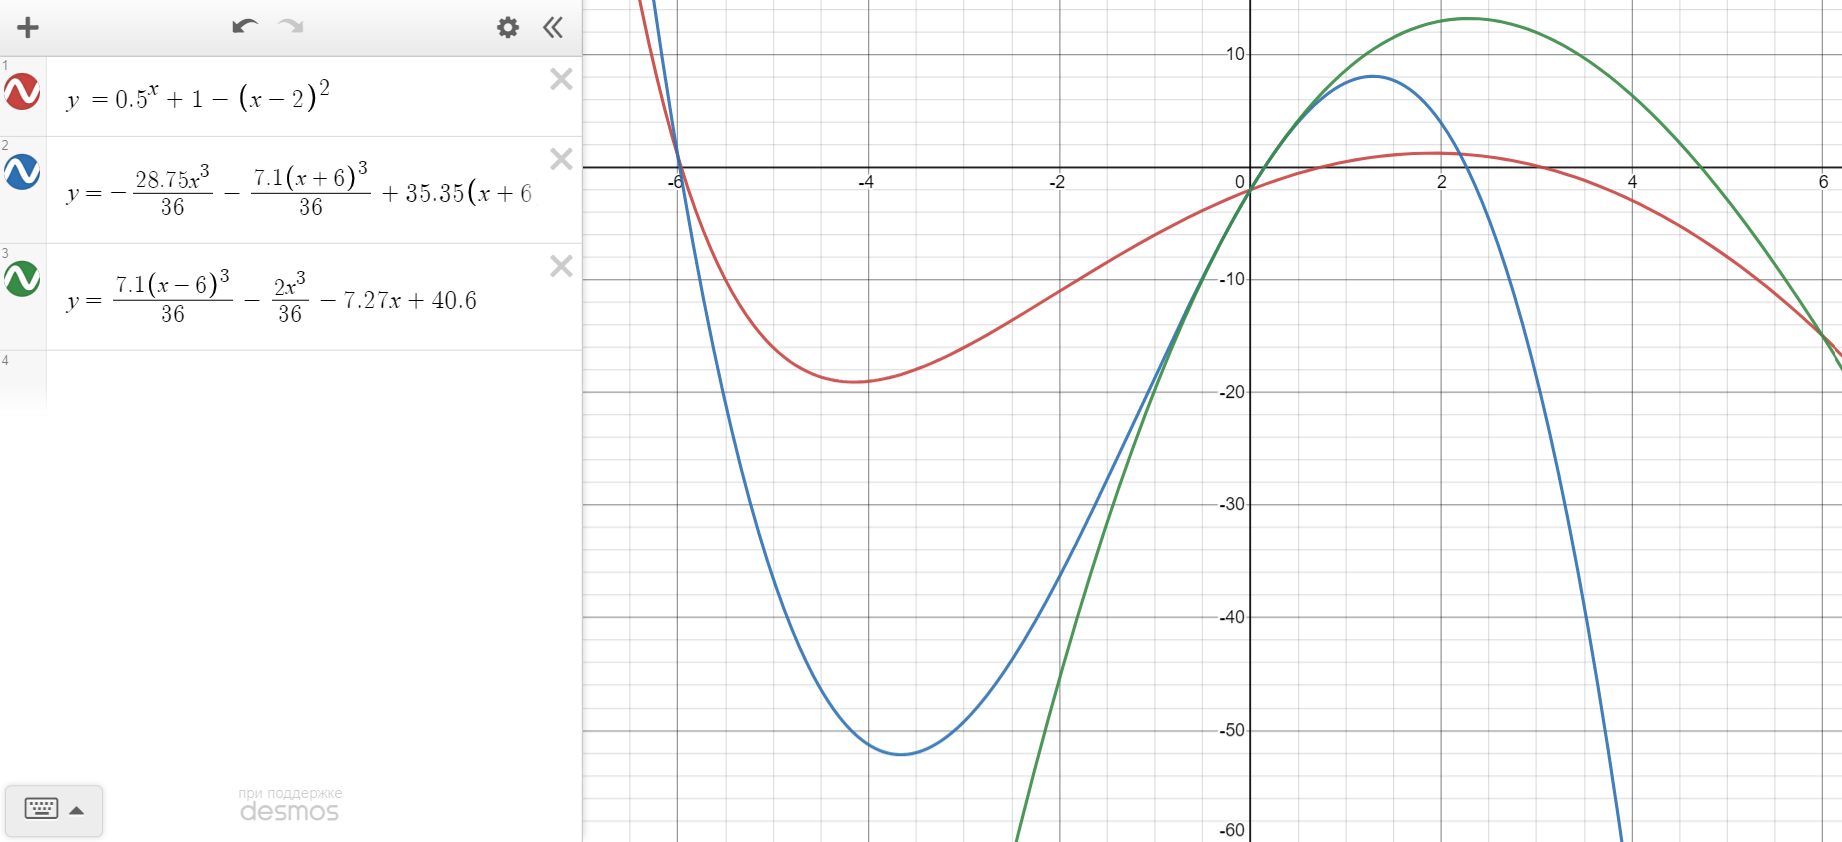
\includegraphics[scale = 0.4]{Тестовый пример}\end{center}
	\newpage
	\begin{center} \textbf{Контрольные тесты}\end{center}
	\begin{enumerate}
		\item Зададим равномерную сетку и построим кубический сплайн дефекта 1 по общей формуле для функции $f(x) = 0.5^x + 1 - (x - 2)^2$, изменяя количество узлов(от 4 до 61).
		\item Зададим равномерную сетку, построим кубический сплайн дефекта 1 для функции $f(x) = 0.5^x + 1 - (x - 2)^2$ для 31 точки и внесем ошибку в значения вторых производных в граничных точках. Будем менять относительную погрешность вносимых ошибок от ($10^{-5}$ до $10^5$).
	\end{enumerate}
	\begin{center} \textbf{Модульная структура программы}\end{center}
	\verb|int GetNum(ifstream *F)|\\
	\verb|double fGetNum(ifstream* F)|\\
	\verb|vector<double> ImportData(ifstream* F, int n)|\\
	- Функции для импортирования данных\\
	\\
	\verb|matrix_t MatrixInit(int size)|\\
	- Функция инициализации матрицы\\
	\\
	\verb|vector<double> ThomasAlgorythm(double h, vector<double> y_i, double a_der,|\\ \verb|double b_der)|\\
	\verb|pair<vector<double>, vector<double>> FindConstants(double h, vector<double> y_i,|\\ \verb|vector<double> M_i)|\\
	\verb|double g_i(double xx, double left_M, double right_M, double left_x, double right_x,|\\ \verb|double C, double C_tilda)|\\
	- Вспомогательные функции для нахождения $M_i$ методом прогонки, констант $C_i$ и $\tilde{C_i}$ и функции $g_i(x)$\\
	\\
	\verb|vector<double> CubicSpline(vector<double> xx, vector<double> x_i, vector<double> y_i,|\\ \verb|vector<double> M_i, pair<vector<double>, vector<double>> C)|\\
	- Реализация кубического сплайна дефекта 1\\
	\\
	\verb|void OutputVector(vector<double> vec, ofstream* F)|\\
	- Функция для экспортирования данных
	\begin{center} \textbf{Численный анализ}\end{center}
	\begin{center}
		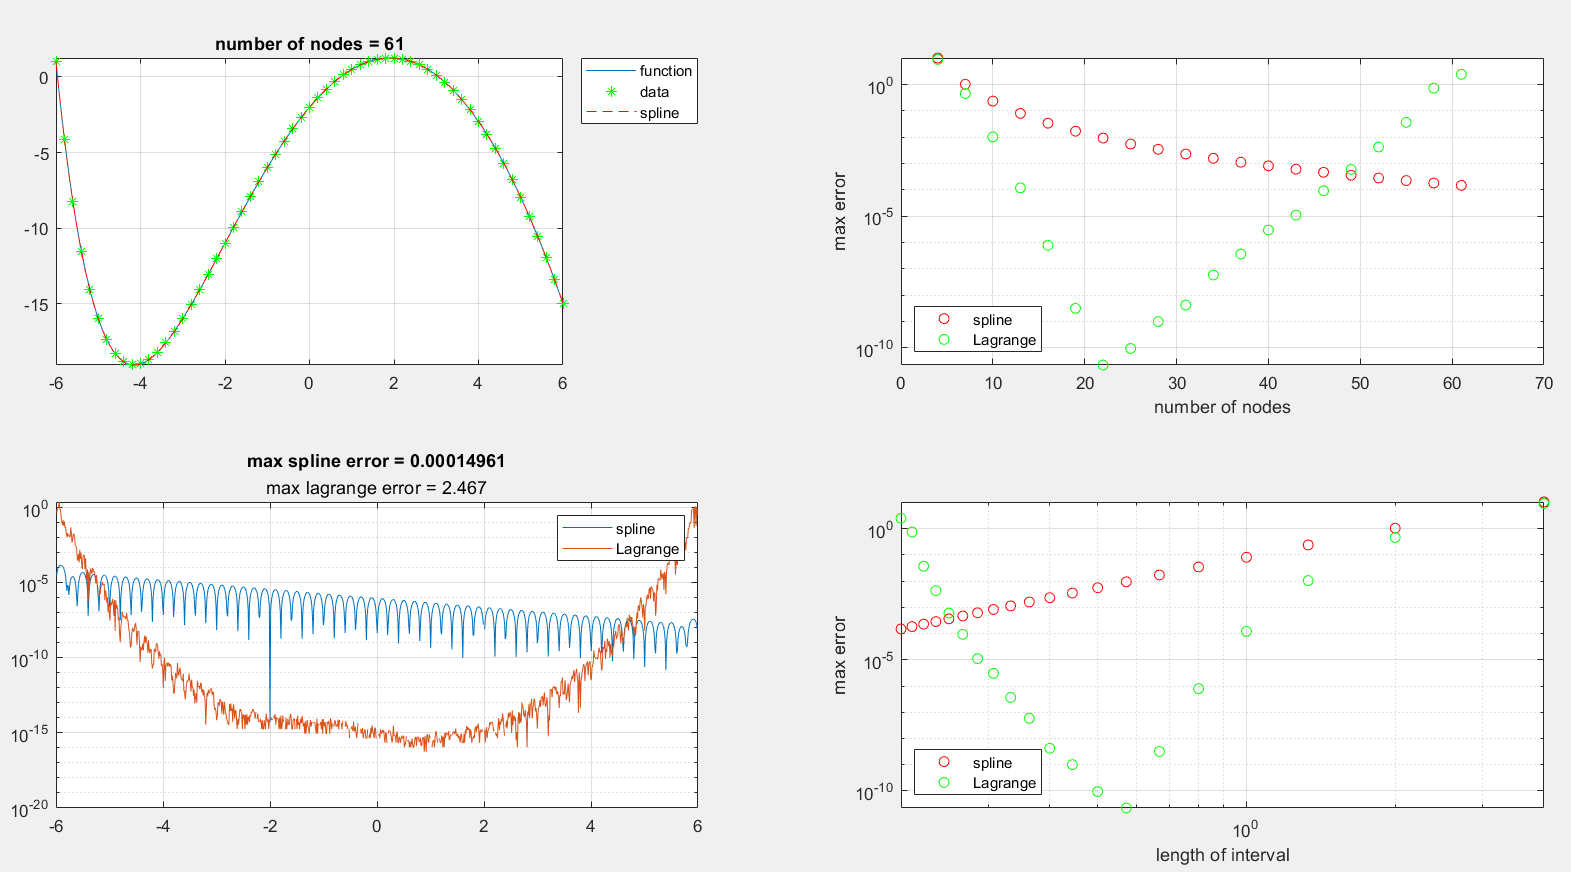
\includegraphics[scale = 0.4]{Приближение}
		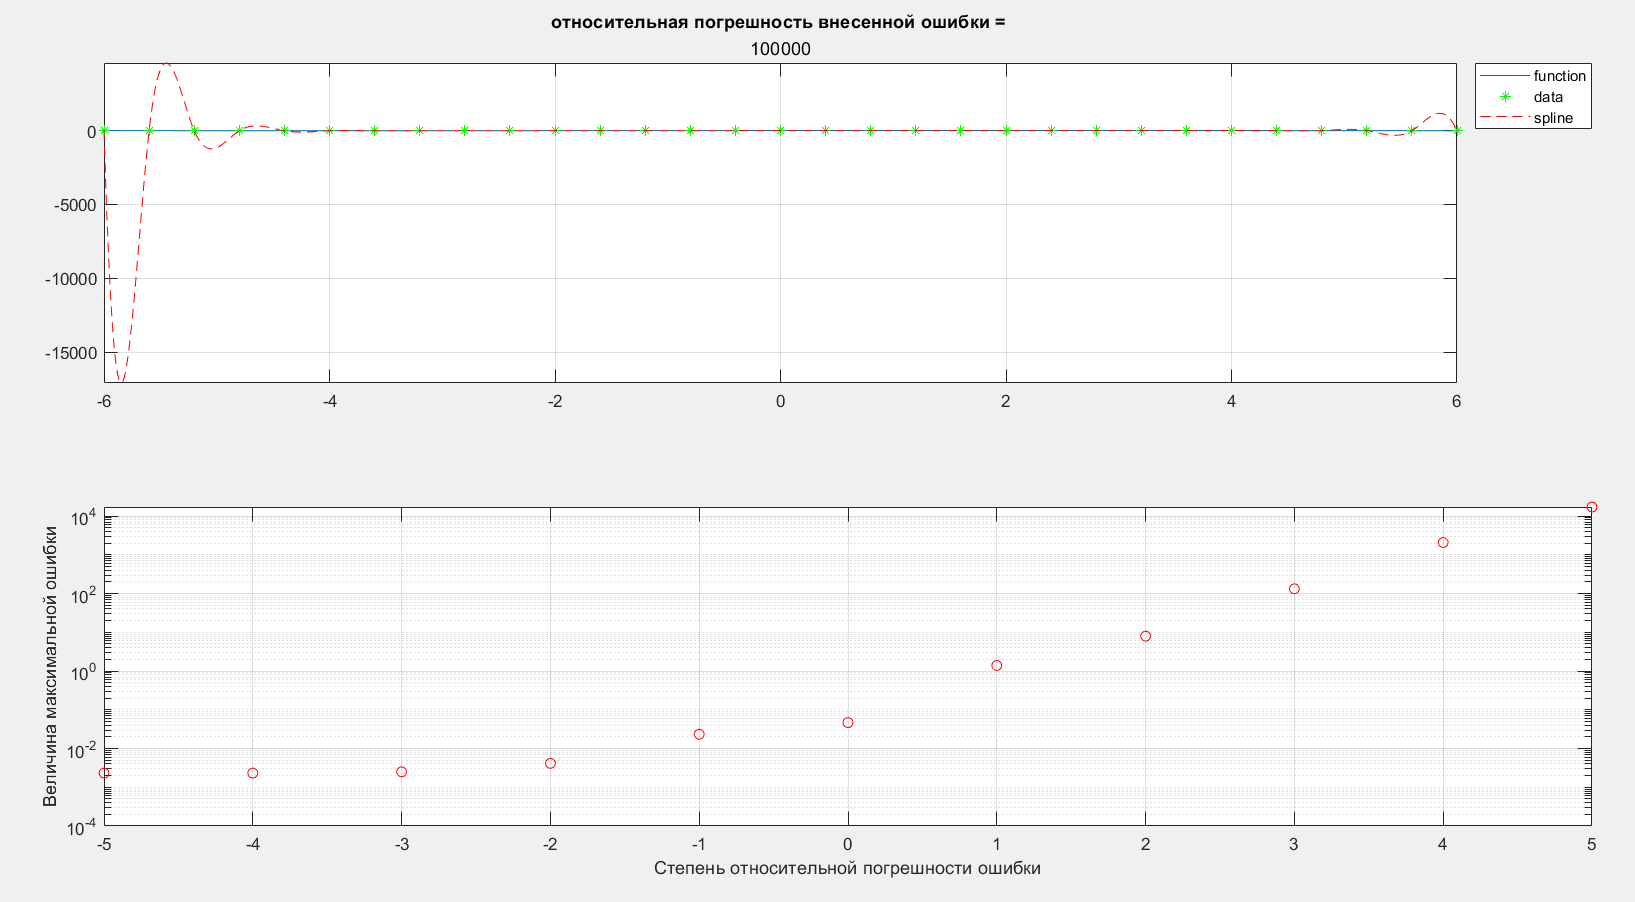
\includegraphics[scale = 0.385]{Ошибка в доп условиях}
	\end{center}
	$\triangleright$ \underline{Приближение:}\\
	При увеличении числа узлов кубический сплайн дефекта 1 все больше и больше становится похож на график функции.\\
	$\triangleright$ \underline{Ошибка:}\\
	Из графика видно, что при малом количестве узлов максимальная ошибка полинома Лагранжа меньше, чем ошибка сплайна, но начиная примерно с 58 узлов она становится больше. Из пооведения графиков ясно, что с этого числа узлов ошибка сплайна всегда будет меньше, поскольку она убывает, а ошибка полинома увеличивается.\\
	$\triangleright$ \underline{Внесенные погрешнности:}\\
	На графике мы видим, что внесение ошибки, относительная величина которой меньше порядка -2, практически не влияет на результат, но затем ошибка начинает увеличиваться.
	\begin{center} \textbf{Общие выводы}\end{center}
	В данной лабораторной работе мы научились апроксимировать сложную функцию кубическими сплайнами. Реализация данного метода довольно легкая, а вычислительная сложность получается порядка $O(n)$, но с большой константой, поэтому такой метод лучше использовать на большем количестве точек.   
\end{document}